\documentclass[20pt, a0paper, landscape]{tikzposter}
\tikzposterlatexaffectionproofoff
\usepackage[utf8]{inputenc}
\usepackage{authblk}
\makeatletter
\renewcommand\maketitle{\AB@maketitle} % revert \maketitle to its old definition
\renewcommand\AB@affilsepx{\quad\protect\Affilfont} % put affiliations into one line
\makeatother
\renewcommand\Affilfont{\Large} % set font for affiliations
\usepackage{amsmath, amsfonts, amssymb}
\usepackage{tikz}
\usepackage{pgfplots}
\usepackage{multicol}
\usepackage{lipsum}
\usepackage{adjustbox}


\usepackage[backend=bibtex]{biblatex}

\usepackage[font=small,labelfont=bf]{caption}
% align columns of tikzposter; needs two compilations
\usepackage[colalign]{column_aligned}
% tikzposter meta settings
\usetheme{Default}
\usetitlestyle{Default}
\useblockstyle{Default}

%%%%%%%%%%% redefine title matter to include one logo on each side of the title; adjust with \LogoSep
\makeatletter
\newcommand\insertlogoi[2][]{\def\@insertlogoi{\includegraphics[#1]{#2}}}
\newcommand\insertlogoii[2][]{\def\@insertlogoii{\includegraphics[#1]{#2}}}
\newlength\LogoSep
\setlength\LogoSep{-70pt}

\renewcommand\maketitle[1][]{  % #1 keys
    \normalsize
    \setkeys{title}{#1}
    % Title dummy to get title height
    \node[inner sep=\TP@titleinnersep, line width=\TP@titlelinewidth, anchor=north, minimum width=\TP@visibletextwidth-2\TP@titleinnersep]
    (TP@title) at ($(0, 0.5\textheight-\TP@titletotopverticalspace)$) {\parbox{\TP@titlewidth-2\TP@titleinnersep}{\TP@maketitle}};
    \draw let \p1 = ($(TP@title.north)-(TP@title.south)$) in node {
        \setlength{\TP@titleheight}{\y1}
        \setlength{\titleheight}{\y1}
        \global\TP@titleheight=\TP@titleheight
        \global\titleheight=\titleheight
    };

    % Compute title position
    \setlength{\titleposleft}{-0.5\titlewidth}
    \setlength{\titleposright}{\titleposleft+\titlewidth}
    \setlength{\titlepostop}{0.5\textheight-\TP@titletotopverticalspace}
    \setlength{\titleposbottom}{\titlepostop-\titleheight}

    % Title style (background)
    \TP@titlestyle

    % Title node
    \node[inner sep=\TP@titleinnersep, line width=\TP@titlelinewidth, anchor=north, minimum width=\TP@visibletextwidth-2\TP@titleinnersep]
    at (0,0.5\textheight-\TP@titletotopverticalspace)
    (title)
    {\parbox{\TP@titlewidth-2\TP@titleinnersep}{\TP@maketitle}};

    \node[inner sep=0pt,anchor=west] 
    at ([xshift=-\LogoSep]title.west)
    {\@insertlogoi};

    \node[inner sep=0pt,anchor=east] 
    at ([xshift=\LogoSep]title.east)
    {\@insertlogoii};

    % Settings for blocks
    \normalsize
    \setlength{\TP@blocktop}{\titleposbottom-\TP@titletoblockverticalspace}
}
\makeatother
%%%%%%%%%%%%%%%%%%%%%%%%%%%%%%%%%%%%%


% color handling
\definecolor{TumBlue}{cmyk}{1,0.43,0,0}
\colorlet{blocktitlebgcolor}{TumBlue}
\colorlet{backgroundcolor}{white}

% title matter
\title{Level 1 Autonomous Driving}

\author[1]{Tom D{\"o}rr}
\author[2]{Theodor Cheslerean Boghiu}
\author[3]{Mohamed asif Chand}
\author[4]{Vlad Paul Cosma}

\affil[1]{tom.doerr@tum.de}
\affil[2]{theo.cheslerean@tum.de}
\affil[3]{mdasifchand@gmail.com}
\affil[4]{vlad.cosma@tum.de}

\insertlogoi[width=15cm]{tum_logo}
\insertlogoii[width=15cm]{tum_logo}

% main document
\begin{document}

\maketitle




\begin{columns}
	
	\column{0.2}
	\block{Semantic Segmentation}{
		\begin{itemize}
\item Definition: Semantic segmentation means assigning a class label to each of the computed segments example: Road, traffic lights, lanes. Examples: Fully CNN(2015), SegNet(2015), ENet(2016), LinkNet(2017). 
\item Semantic Segmentation is used to detect road in the absence of clear road-lane separation
\item Present developments in Semantic Segmentation on autonomous vehicles
   \subitem SqueezeNet(2016) was able to demonstrate the increase in accuracy of AlexNet using 50 times less parameteres by tweaking with the architectures
   \subitem ENet(2016) could replicate the Semantic Segmentation on real time
\end{itemize}
  \begin{minipage}{0.16\textwidth}
\centering
  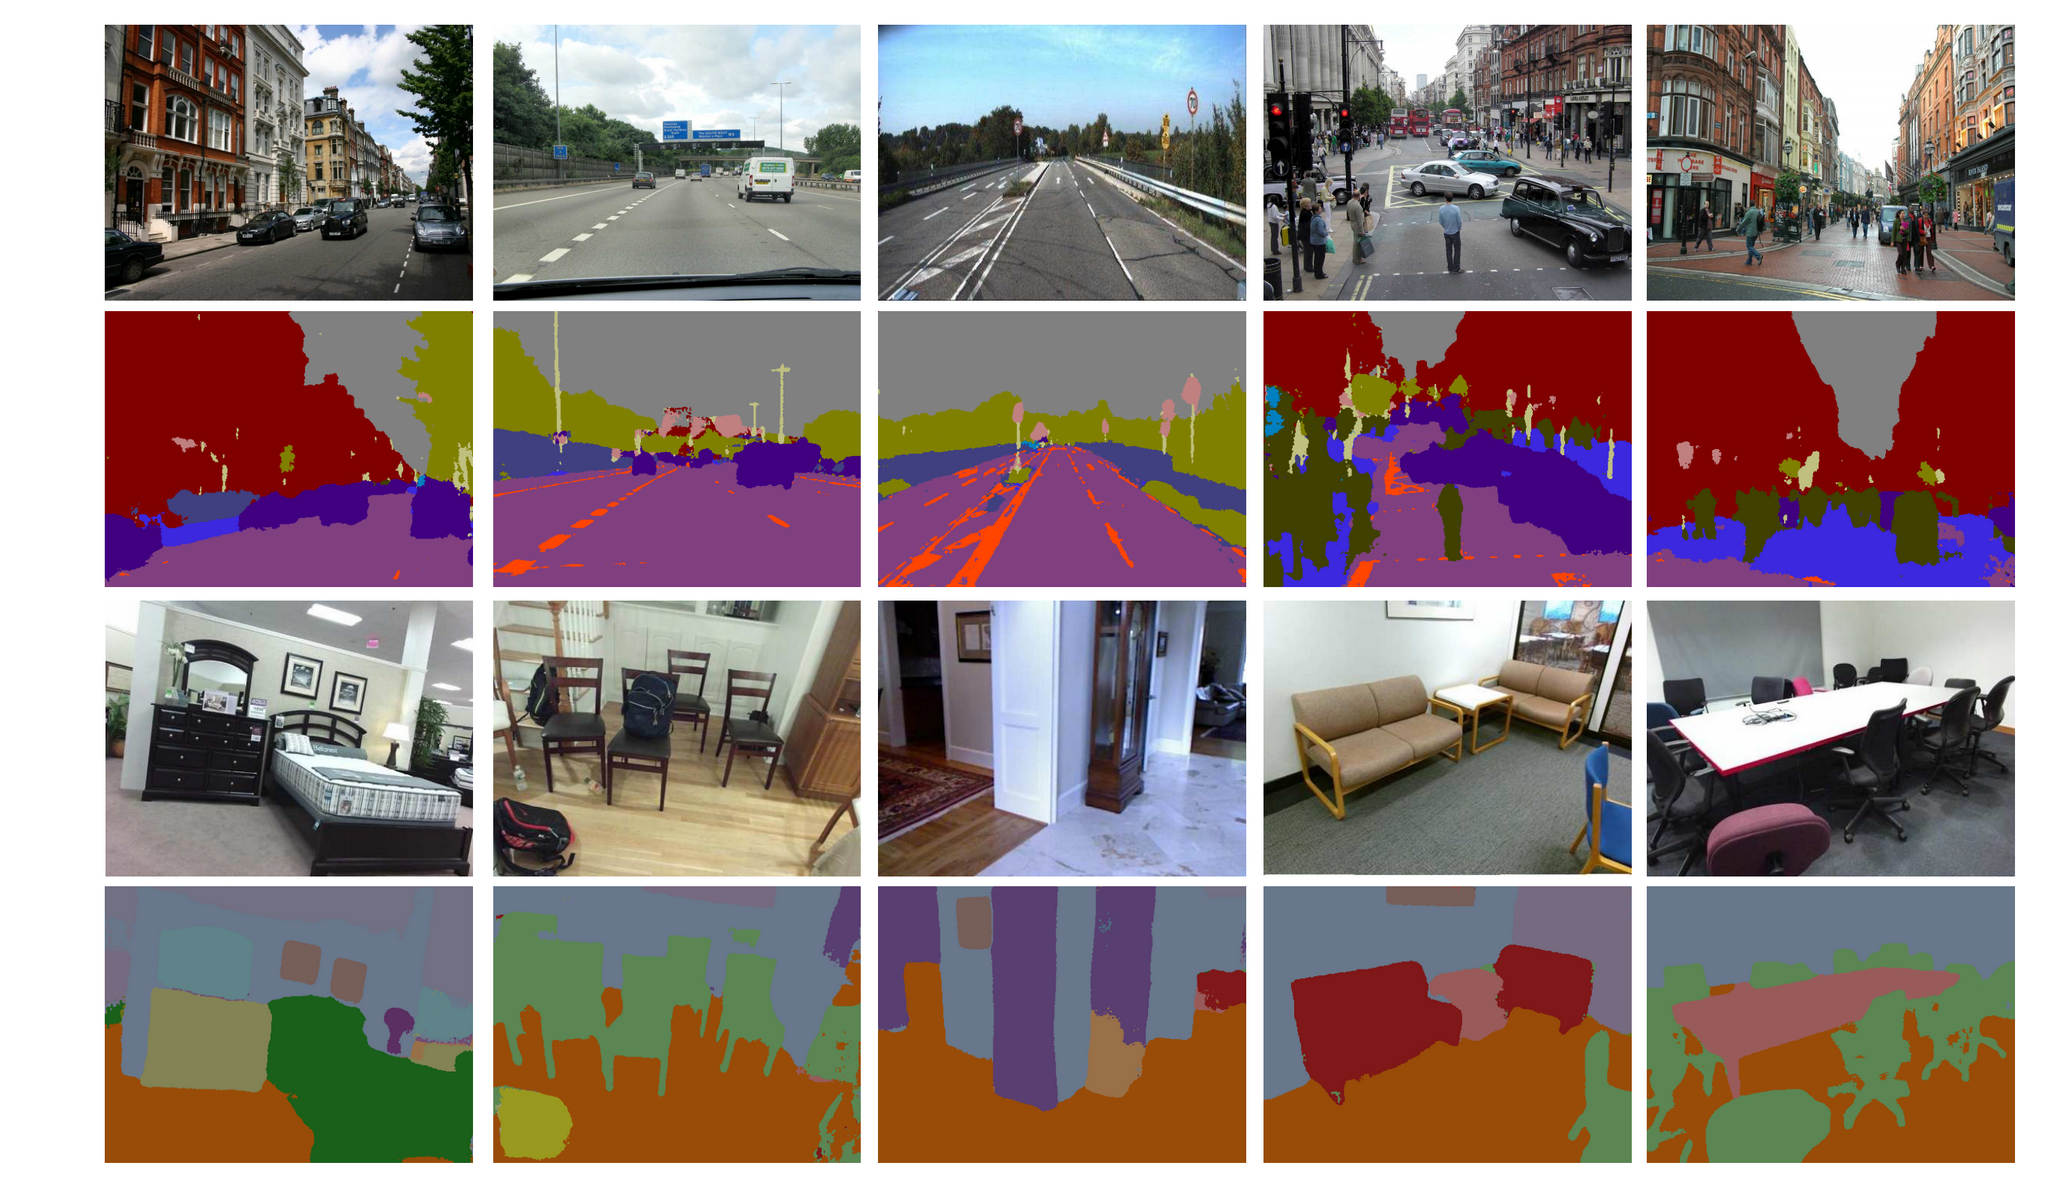
\includegraphics[width=0.65\linewidth]{images/scr1.png}
  \captionof{figure}{Segnet predictions on road scene and indoor scenes}
\end{minipage}  
  

	}

	\block{Udacity Simulator \textsuperscript{4}}{	
		Udacity provides a free and easy to use platform for testing and gathering data in autonomous driving tasks.
It encompasses the following set of features:
\begin{itemize}	
	\item Compatible with both Windows and Linux systems(compared to GTA V)
	\item Built-in
		\subitem Data Collection Mode
		\subitem Autonomous Driving Mode
	\item Customizable through Unity
\end{itemize}
The data gathering is done by capturing the screen output and the steering angle input from a user. This data is saved in the form of the screenshots, each one annotated with the steering angle value, which can then be used for training.
	}

	\column{0.6}

	\block{Cityscapes Dataset \textsuperscript{3}}{
		\begin{multicols*}{2}
The cityscape dataset is used for the semantic segmentation part of our project. It encompasses the following features:
\begin{itemize}	
	\item 30 class definitions related to city driving
	\item Various weather conditions
	\item 25000 annotated images
	\item Metadata including: GPS coordinates, Odometry data of ego vehicle, Preceding and trailing video frames
\end{itemize}
\begin{minipage}{0.25\textwidth}
\centering
  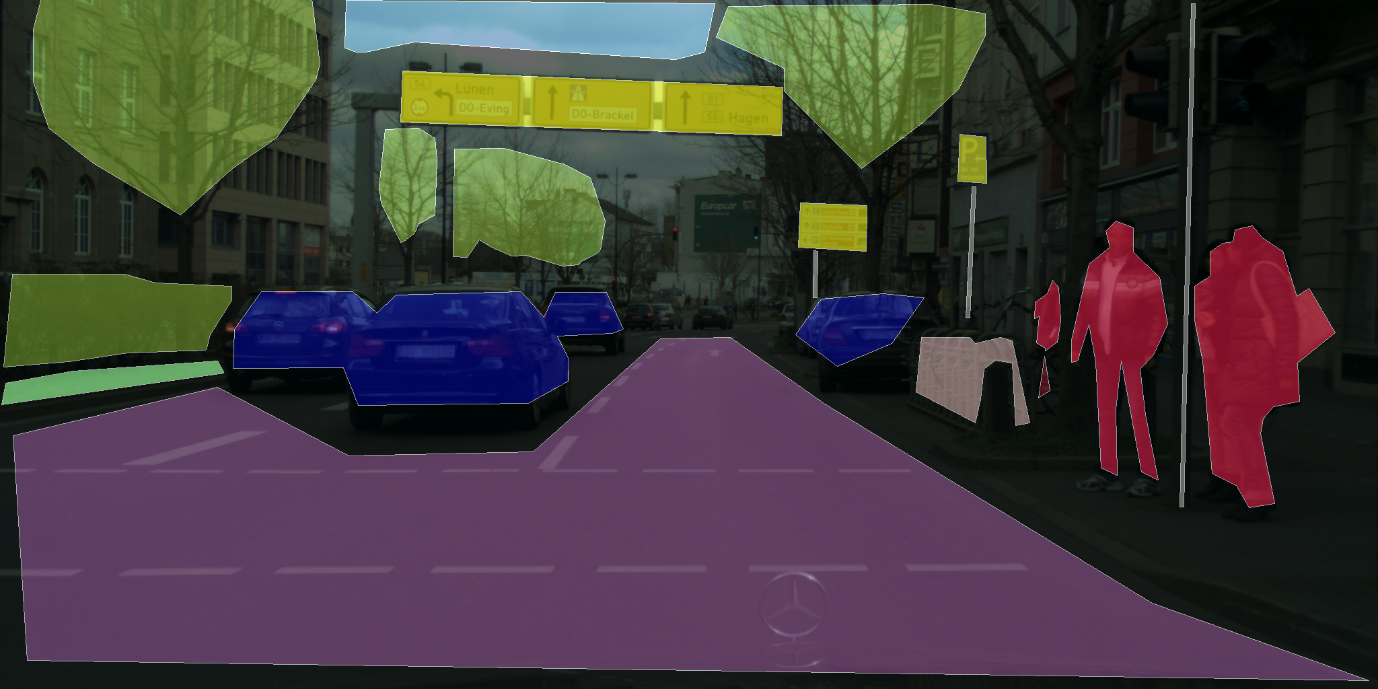
\includegraphics[width=0.5\linewidth]{images/cityscapes_dataset.png}
  \captionof{figure}{Cars - blue, Pedestrians - red, Road - purple, Sidewalk – light green, Vegetation – green, Traffic signs - yellow, Guard rail – light brown}
\end{minipage}
\end{multicols*}
	}
	\block{Segmentation Architecture \textsuperscript{2}}{
		\begin{multicols*}{2}
\begin{itemize}
\item The architecture selected for the problem definition was taken as SegNet(2015) because of it's simplicity 
\item Transfer training of the weights is performed and then fine tuned to attain the segmentation of the road. 
\end{itemize}
\begin{minipage}{0.25\textwidth}
\centering
  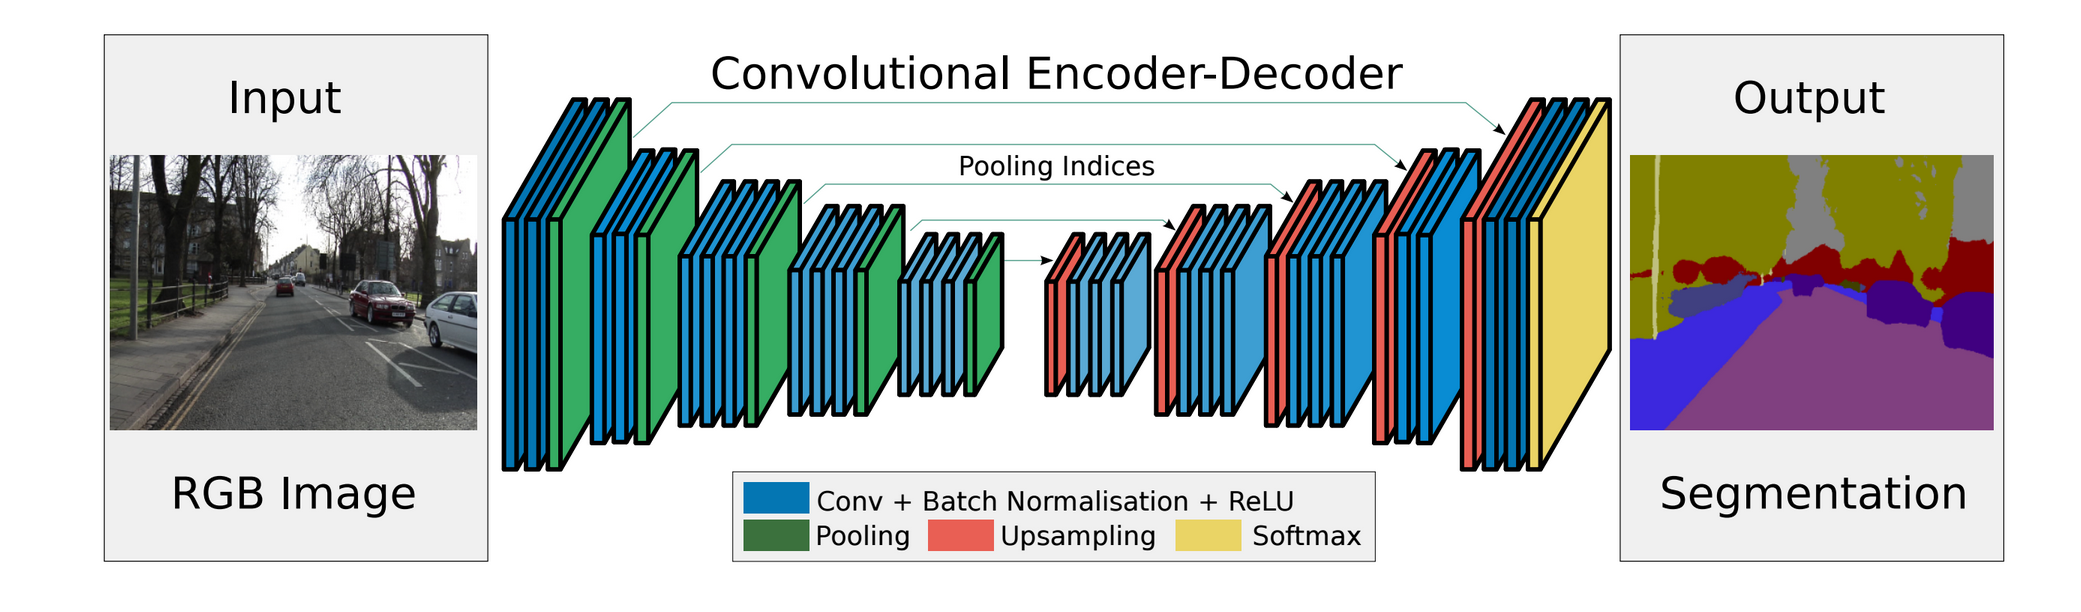
\includegraphics[width=0.75\linewidth]{images/scr2.png}
  \captionof{figure}{SegNet does not include any fully connected layer hence it is only convoluted. A sparse map of features is produced by the decoder which upsamples input produced by the encoder using encoders transferred pool indices. Then performs convolution with a trainable filter bank to densify the sparse feature map. Softmax classifier takes the final decoder output for pixel wise classification }
\end{minipage}
\end{multicols*}
	}
	\block{Udacity Dataset}{
		\begin{multicols*}{2}
The udacity dataset is created from the udacity car simulator. It associate via a timestamp 3 images taken at an offset (left, center and right) with steering angles, brake and acceleration. Our dataset contains 8036 frames of the simulation game along with odometry information. These images have been resized and modified in the following way randomly in order to increase the model’s prediction capacity: 
\begin{itemize}	
	\item Randomly chosen from an offset (left, center, right)
	\item Brightness changed
	\item Cropped
	\item Shadow mask added
	\item Flipped (left becomes right and right becomes left)
	\item Translated (shift the image vertically and horizontally)
	\item RGB 2 YUV (YUV is a color space more closely related to human perception)
\end{itemize}
All of the preprocessing is done using the python opencv library.
\\
\begin{minipage}{.25\textwidth}
	\centering
	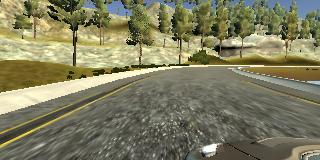
\includegraphics[width=0.2\linewidth]{images/left_image.png}
	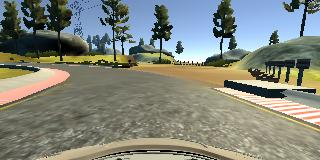
\includegraphics[width=0.2\linewidth]{images/center_image.png}
	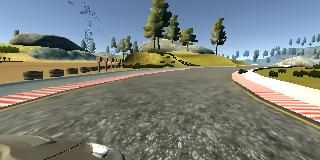
\includegraphics[width=0.2\linewidth]{images/right_image.png}
	\captionof{figure}{Left, Center and Right Image}
\end{minipage}
\end{multicols*}
	}
	\block{Nvidia Architecture}{
		\begin{multicols*}{2}
A modified version of the Nvidia model is used\textsuperscript{1}.

We're leaving out one fully connected layer and cut the number of Convolutional
feature maps in halve. We still have the last 3 fully connected layers and
 also have the five convolutional layers of the original network. As an activation function we are using ELU.
\begin{minipage}{0.25\textwidth}
 \centering
  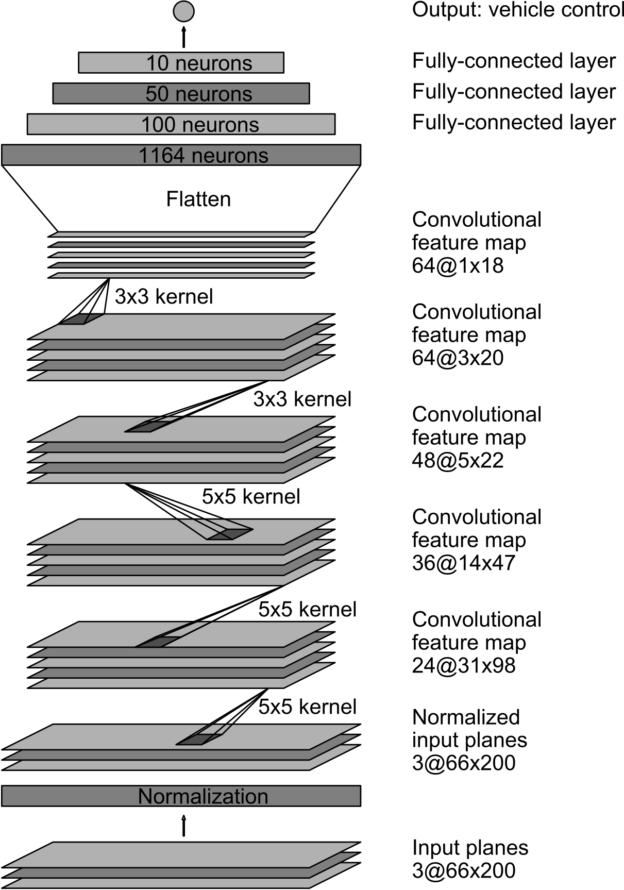
\includegraphics[width=0.75\linewidth, height=0.1\linewidth]{images/nvidia_architecture.png}
  \captionof{figure}{Cars - blue, Pedestrians - red, Road - purple, Sidewalk – light green, Vegetation – green, Traffic signs - yellow, Guard rail – light brown}
\end{minipage}
\end{multicols*}
	}

	\column{0.2}
	\block{Segmentation Training Results}{\phantom{Q\\Q\\Q}}
	\block{Segmentation Testing Results}{\phantom{Q\\Q\\Q\\Q\\Q}}

	\block{Driving Training Results}{\phantom{Q}}
	\block{Driving Testing Results}{\phantom{Q\\Q\\Q}}
\end{columns}

\block{References} {
%\begin{multicols*}{4}
\textsuperscript{1} https://devblogs.nvidia.com/parallelforall/deep-learning-self-driving-cars/
\textsuperscript{2} SegNet: A Deep Convolutional Encoder-Decoder Architecture for Image Segmentation by Vijay Badrinarayanan et.al
\textsuperscript{3} https://www.cityscapes-dataset.com/
\textsuperscript{4} https://github.com/udacity/self-driving-car-sim
%\end{multicols*}
}

\end{document}